\section{Mapping and navigation}
In order to navigate in the maze three map layers are used. The first layer is an occupancy grid, which is based on data from the IR sensors. The second layer is something we call the ``seen map'' which is an estimation of which areas of the map that the primesense has seen. The third layer is a topological map.

\subsection{Occupancy grid}
An occupancy grid is essentially a matrix where each cell is either occupied, free or unknown. 
The internal representation contains the probability that a cell is occupied in log odds notation \cite{wiki:Logit}.
An unknown cell contains our prior belief that a cell is occupied, in our model that was $l(0.5)$, i.e. it is as likely to be occupied as free. 
Any cell with a value higher than the prior is considered to be occupied, and any cell with a smaller value is considered to be free.

When a cell is within the field of view of an IR sensor the probability of that cell being occupied is update according to the following fomula:

\begin{equation}
p_{x, y} = p_{x, y} + p_{new} - p_{prior}
\end{equation}

where $p_{new}$ is the tentative belief that the cell is occupied. By taking previous observations in to account, the model is less sensetive to sensor noise. \cite{GridLecture}

The grid has a resolution of one cell per square centimater, and a fixed size of 1000 by 1000 cells. 
The robot always starts in the middle of the grid, which means that it can go five meters in any direction without going out of bounds, which was enough.

The main useage of the occupancy grid is when a new node is placed in the topological map. 
In order to decide which directions of the new node contain unexplored space the occupancy grid is used in combination with the seen map. 
A direction is considered unexplored if the ratio of occupied cells and seen cells is below the respective thresholds.

\subsection{Seen map}
The ``seen map'' is a map which contains an estimation of which areas of the map that the primesense has seen. 
It is implemented by marking a circular sector as seen in front of the robot in each time step. 
As previously stated, it is used in conjunction with grid map to decide which areas of the map are unexplored. 
This saves us a lot of unnecessary exploration.

\subsection{Topological map}
The topological is our primary tool for navigation. Nodes are placed when the robot encounters an obstacle, when an intersection is detected, when an object is recognized, and at the starting position. When a node is placed the four compass directions (north, east, south and west) are marked as either unexplored or blocked, according on the previously stated condition. This does not apply to the direction from which we came, which is connected to the previous node instead. When we return to a node a connection is also made to the previous node.

To navigate in the maze the topological map offers a service that let's the master node navigate to the next point of interest, which can be either an unexplored area, or an object, depending on which mode is activated. Dijkstra's algorithm is used to find the shortest path.

\begin{figure}[h]
\begin{center}
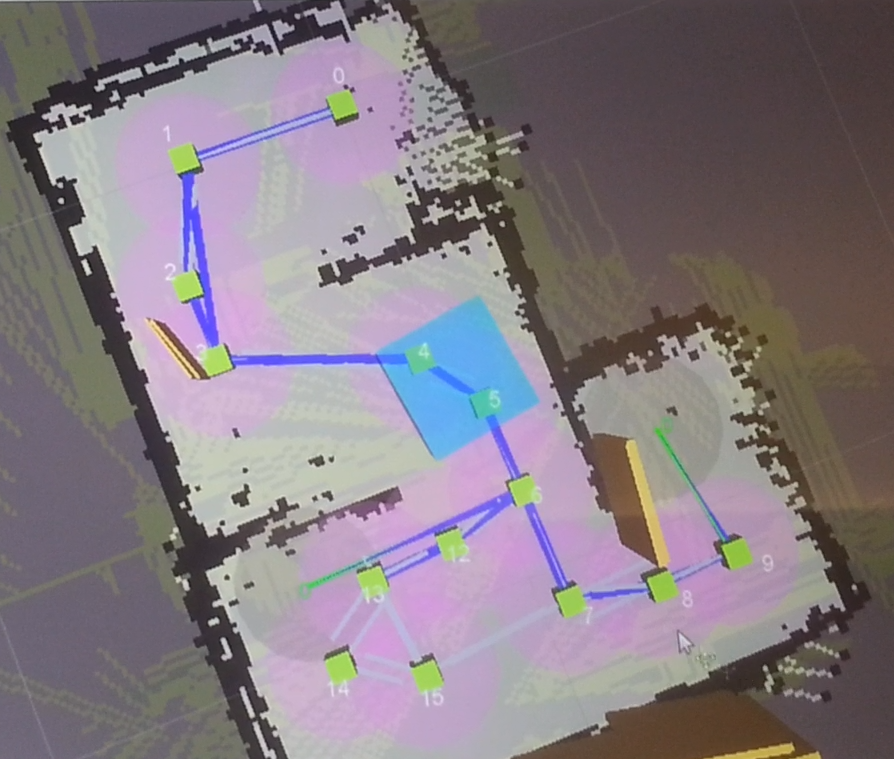
\includegraphics[width=0.6\textwidth]{figures/map.png}
\end{center}
\caption{A screenshot of all map layers in rviz. The robot is the large cube. Nodes are represented by the small cubes (except objects, which are the points with an edge to them without a cube). The have seen map is represented by the yellowish lines. In this image the robot is running phase two. It has recognized two objects, returned to the start, and is now on its way to fetch the objects. The edges that make up the TSP tour are blue.}
\label{fig:arch_controller}
\end{figure}

\subsection{Path following}
Although an actual controller, the path follower (in figure \ref{fig:1st_architecture} the top most instance called \textit{Goto}),
takes a path of points in the map, optimizes and follows it.
Because the path follower is going node by node, resulting in stops at every node, the optimization is necessary to reduce the travel time.
It is done by doing a greedy approach of removing nodes that can be skipped because the path between them is obstacle free.
For that a raycast service was implemented in the mapping, that traces a ray for a given distance and checks for obstacles.
Due to some noise in the grid map, it did not perform as well as expected.